\section{Objetivo}
Conocer el funcionamiento de los algoritmos genéticos, su aplicación, pros y contras.\par
Entender los mecanismos de herencia, mutación, selección y cruza, así como su relación con la selección natural.
Implementar un algoritmo genético que resuelva y optimice un problema dado.

\begin{auxcode}
 \caption{Algoritmos genéticos}
 \centering
 \hurl{\auxprefix ia-algoritmos-geneticos}
\end{auxcode}

\section{Introducci\'on}

Un algoritmo genético es una heurística de búsqueda que está basada en el proceso de \textbf{selección natural}.  Su objetivo es encontrar soluciones óptimas a problemas combinatorios. La selección natural es un proceso gradual mediante el cual las características biológicas se vuelven más o menos comunes en una población. Esto depende de las características heredadas y de la diferencia de éxito reproductivo de los organismos que interactúan con su entorno. La selección natural es el mecanismo clave de la \textbf{evolución}. El término de “selección natural” fue popularizado por Charles Darwin desde el año de 1859.

\subsection{Metodolog\'ia}

En un algoritmo genético, una \textbf{población} de candidatos a solución (también llamados \textbf{individuos} o fenotipos) es evolucionada para obtener soluciones óptimas del problema. Cada individuo tiene una representación (sus cromosomas o genotipo) que puede ser alterada o mutada; tradicionalmente, las representaciones son cadenas binarias de 0’s y 1’s, pero otras representaciones son posibles.\par

La evolución es un proceso iterativo mediante el cual se generan individuos aleatoriamente para crear otra población en cada iteración, llamada \textbf{generación}. En cada generación, la \textbf{aptitud} (\textit{fitness}) de cada individuo es evaluada. Usualmente la aptitud es el valor de la función objetivo del problema de optimización que se quiere resolver. Se seleccionan de manera aleatoria individuos de la población para que modifiquen su genoma, \textbf{recombinando} y posiblemente \textbf{mutando} aleatoriamente sus componentes para formar una nueva generación. La nueva generación de posibles soluciones es usada en la siguiente iteración del algoritmo. Comúnmente, el algoritmo termina cuando se alcanza el número máximo de iteraciones o el valor de aptitud de un individuo se ha aproximado lo suficiente a un valor óptimo.

\subsection{Requisitos del algoritmo gen\'etico}

\begin{enumerate}
  \item Una \textbf{representación} genética del dominio de la solución.
  \item Una \textbf{función de aptitud} (\textit{fitness}) a evaluar sobre el dominio de la solución.
\end{enumerate}

\noindent La representación estándar de cada individuo es un arreglo de bits, sin embargo, arreglos de otro tipo y estructuras funcionan esencialmente de la misma manera. El motivo por el cual se prefiere la representación estándar es porque facilita las operaciones de recombinación debido a la longitud fija del arreglo, también la operación de mutación se vuelve trivial como se notará más adelante.


\subsection{Etapas del algoritmo gen\'etico}

\subsubsection{Inicializaci\'on}

Usualmente se genera una cantidad de soluciones posibles de manera aleatoria para formar la población inicial. El tamaño de la población depende del problema y puede llegar a contener cientos de miles de individuos.

\subsubsection{Selecci\'on}

La selección es una etapa del algoritmo genético en la cual se selecciona un individuo de la población que después será recombinado con otro.\par

Existen diferentes maneras de realizar el proceso de selección, el más común es la \textbf{selección proporcional de aptitud} (selección de ruleta). En este tipo de selección, la aptitud (o \textit{fitness}) del individuo se asocia con su probabilidad de selección.\par

Entonces si \(f_i\)  es la aptitud del individuo \(i\) en la población, la probabilidad de ser seleccionado es:\par
\[p_i = {f_i \over \sum_{j=1}^{N} f_j}\]
donde \(N\) es el número de individuos en la población.\par

Esto es similar a imaginar una ruleta de casino. Usualmente una proporción de la rueda de la ruleta es asignada a cada posible individuo basado en su aptitud. Esto se logra al dividir la aptitud de cada individuo entre el total de aptitud de todos los individuos, que es equivalente a normalizarlos a 1. Entonces un individuo es aleatoriamente seleccionado de la manera en que lo haría una ruleta que está girando.

\subsubsection{Operadores gen\'eticos}

\paragraph{Recombinaci\'on}

La recombinación es el operador genético que permite la variación de cromosomas de los individuos de la población de una generación a otra. Es análoga a la reproducción y la recombinación biológica. El proceso de recombinación consiste en tomar más de un individuo y producir un nuevo hijo o solución.\par

Hay varias técnicas de recombinación, la más habitual es la recombinación de un punto y consiste en seleccionar aleatoriamente un mismo punto de corte dentro de la cadena de cromosomas de los padres e intercambiar su contenido para generar nuevos hijos:

\begin{figure}[H]
  \centering
  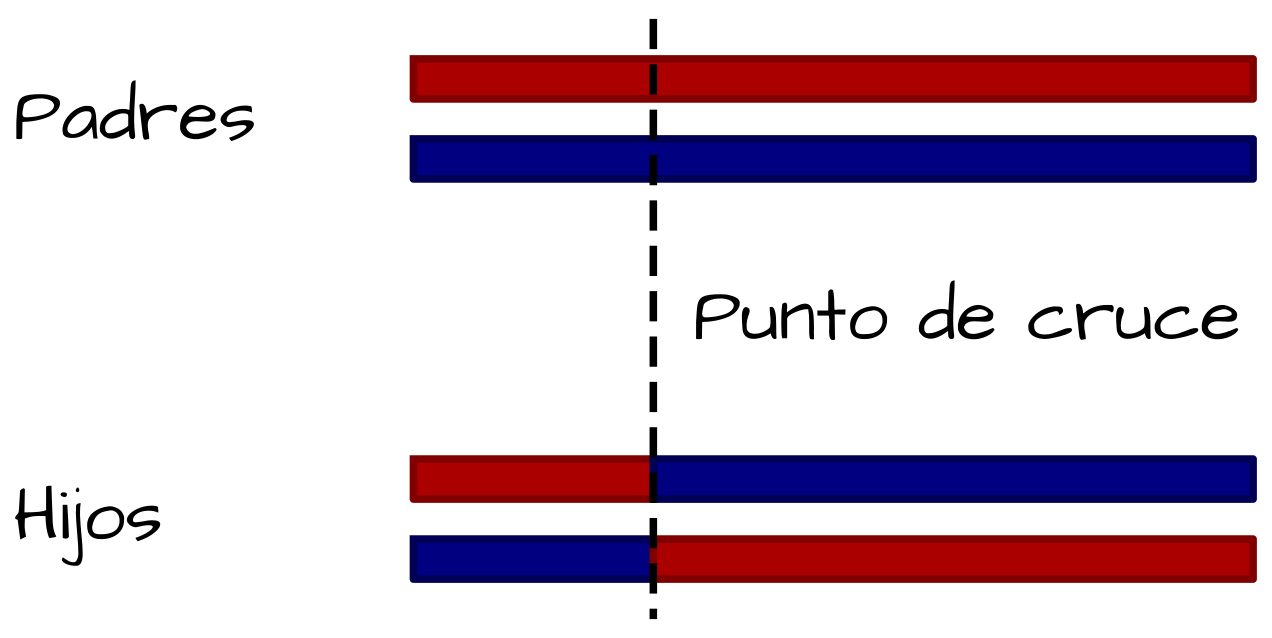
\includegraphics[scale=0.6]{geneticos/cruce.png}
  \caption{Operación genética recombinación de un punto.}
\end{figure}

\begin{table}[H]
  \centering
  \begin{tabular}{|l|l|}
  \hline
  Padre 1 & \textcolor{red}{1 1 0 1 0 0 1 0 0 1 1 0 1 1 0}                    \\ \hline
  Padre 2 & \textcolor{blue}{1 0 0 1 1 1 0 1 1 0 0 1 0 1 1}                   \\ \hline
  Hijo 1  & \textcolor{red}{1 1 0 1} \textcolor{blue}{ 1 1 0 1 1 0 0 1 0 1 1} \\ \hline
  Hijo 2  & \textcolor{blue}{1 0 0 1} \textcolor{red}{0 0 1 0 0 1 1 0 1 1 0}  \\ \hline
  \end{tabular}
  \caption{Ejemplo numérico de recombinación.}
\end{table}

\paragraph{Mutaci\'on}

La mutación es el operador genético que mantiene la diversidad genética de una generación a otra, de manera análoga a la mutación biológica. La mutación altera uno o más de los genes (valores) en el cromosoma. Esta alteración puede cambiar por completo la solución antes de aplicar el operador de mutación y puede llegar a obtener mejores soluciones (o peores) dentro del algoritmo genético.\par

Las mutaciones ocurren valor por valor en un individuo de acuerdo a una probabilidad de mutación que es definida por el usuario. Esta probabilidad debería ser baja porque si se establece un probabilidad de mutación muy alta el algoritmo genético se convierte en una búsqueda de soluciones de manera aleatoria.

\begin{table}[H]
  \centering
  \begin{tabular}{|l|l|}
  \hline
  Cromosoma original & 1 1 0 1 \textcolor{red}{0} 0 1 0 0 1 1 0 1 \textcolor{red}{1} 0  \\ \hline
  Cromosoma mutado   & 1 1 0 1 \textcolor{red}{1} 0 1 0 0 1 1 0 1 \textcolor{red}{0} 0  \\ \hline
  \end{tabular}
  \caption{Ejemplo del operador de mutación.}
\end{table}

\subsubsection{Terminaci\'on del algoritmo}

Las iteraciones del algoritmo genético se terminan hasta que se alcanza alguna de las condiciones de terminación, que pueden ser:

\begin{itemize}
  \item Una solución es encontrada tal que satisface un criterio mínimo.
  \item Un número fijo de generaciones ha sido alcanzado.
  \item Se alcanza el máximo de los recursos posibles (por ejemplo: tiempo de procesamiento).
  \item Se alcanza el valor de aptitud más alto posible o se llega a un estado en el cual las iteraciones sucesivas no producen mejores resultados (puede deberse a la falta de diversidad, por ejemplo).
  \item Al hacer una inspección manual.
  \item O combinaciones de las anteriores.
\end{itemize}



\subsubsection{Elitismo}

Hay muchas variaciones que pueden hacerse a un algoritmo genético, una de ellas es el proceso de elitismo. Esta variante permite que algunas de las mejores soluciones pasen a la siguiente generación sin alteraciones por recombinación ni mutación.


\section{Desarrollo e implementaci\'on}

Se desea resolver el problema de las ocho reinas mediante algoritmos genéticos.  Este problema consiste en colocar ocho reinas del juego de ajedrez en un tablero de \(8 \times 8\) de tal manera que no se ataquen mutuamente. Entonces, encontrar una solución requiere que entre cualesquiera dos reinas no compartan columna, fila, ni diagonal entre ellas. El problema de las ocho reinas es un caso particular de otro más general, el de las \(n\)-reinas, que consiste en colocar \(n\) reinas en un tablero de dimensiones \(n \times n\).

\begin{figure}[H]
  \centering
  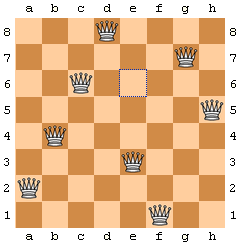
\includegraphics[scale=0.5]{geneticos/8queens.png}
  \caption{Ejemplo de solución al problema de las ocho reinas. \protect\footnotemark}
  \label{fig:queens}
\end{figure}
\footnotetext{https://matteoredaelli.wordpress.com/2009/01/05/n-queens-solution-with-erlang/}

\subsection{Consideraciones de la implementaci\'on}

\subsubsection{Representaci\'on gen\'etica}\par

Es recomendable emplear una representación de un tablero mediante una arreglo de números que identifica la posición por filas de cada reina.
Esta representación es muy conveniente porque evita que las reinas se ataquen por filas y facilita el proceso de encontrar una solución.

\begin{figure}[H]
  \centering
  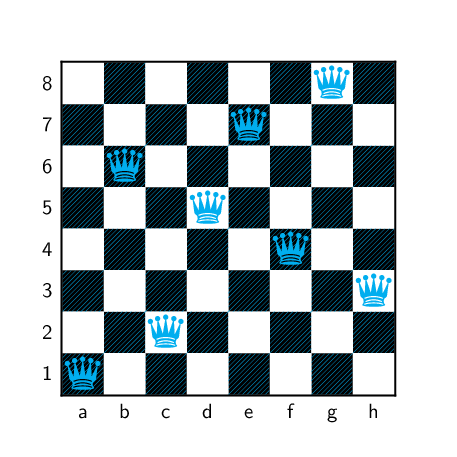
\includegraphics[scale=0.3]{geneticos/NReinas.png}
  \caption{La representación del tablero sería [1, 6, 2, 5, 7, 4, 8, 3].}
  \label{fig:P8screen2}
\end{figure}


\subsubsection{Funci\'on de aptitud}\par

La optimización que se desea es encontrar un tablero en donde las reinas no se ataquen, de manera que la función de aptitud es inversamente proporcional a la cantidad de ataques entre reinas en un tablero.
La figura~\ref{fig:P8screen2} muestra un tablero donde sólo existe un ataque entre reinas, casi es un tablero óptimo por lo que el resultado de la función de aptitud debe ser un valor alto.

\subsubsection{Operador de recombinaci\'on}

Se utilizará el operador de corte de un punto eligiendo aleatoriamente un punto de corte, ilustrado con el siguiente ejemplo:

\begin{figure}[H]
  \centering
  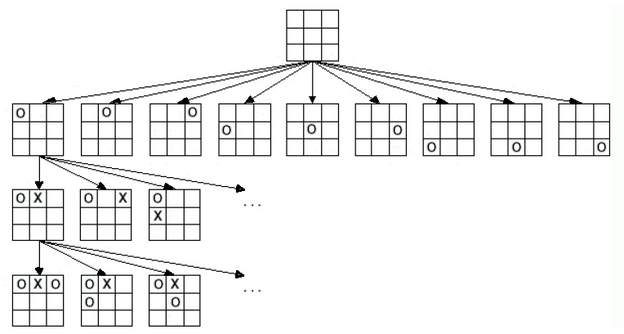
\includegraphics[scale=0.6]{geneticos/screen3.png}
  \caption{Recombinación de dos tableros para producir un nuevo tablero hijo.}
\end{figure}


\subsubsection{Operador de mutaci\'on}

El operador de mutación será definido con una probabilidad de mutación de 0.2. Es decir, se recorrerá cada gen del cromosoma (cada número del arreglo) y se modificará su valor con probabilidad 0.2.

\begin{table}[H]
  \centering
  \begin{tabular}{|l|l|}
  \hline
  Tablero original & {[} 8, 3, 7, 4, 2, \textcolor{red}{5}, 1, 6 {]}  \\ \hline
  Tablero mutado   & {[} 8, 3, 7, 4, 2, \textcolor{red}{3}, 1, 6 {]}  \\ \hline
  \end{tabular}
  \caption{Ejemplo de mutación para un tablero de ajedrez.}
\end{table}

\subsubsection{Selecci\'on}

Se utilizará el método proporcional de selección por ruleta descrito anteriormente.

\subsubsection{Terminaci\'on del algoritmo}

El algoritmo genético debe terminar cuando encuentra una solución óptima (sin ataques entre reinas) o cuando se hayan alcanzado 1000 generaciones.

\subsubsection{Cantidad de poblaci\'on}

La población de cada generación estará constituida por 50 individuos.

\subsubsection{Elitismo}

Para asegurarnos de mantener al menos una solución lo suficientemente buena, se utilizará elitismo de 1 individuo en cada generación.

\subsection{Pseudoc\'odigo}

El comportamiento general del algoritmo genético puede representarse a través del siguiente pseudocódigo:\medskip

\begin{algorithm}
\caption{Algoritmo genético}
\begin{algorithmic}
  \State $poblaci\acute{o}n\gets new Poblaci\acute{o}n(50)$
  \State $poblaci\acute{o}n.asignarAptitud()$
  \While{not $limiteDeGeneraciones$ or $\acute{o}ptimoEncontrado$}
    \State $nuevaPoblaci\acute{o}n.add(poblaci\acute{o}n.elitismo(1))$
    \While{not $nuevaPoblaci\acute{o}n.llena$}
      \State $individuo1\gets poblaci\acute{o}n.seleccionRuleta()$
      \State $individuo2\gets poblaci\acute{o}n.seleccionRuleta()$
      \State $hijo\gets recombinaci\acute{o}n(individuo1, individuo2)$
      \State $hijo.mutaci\acute{o}n()$
      \State $nuevaPoblaci\acute{o}n.add(hijo)$
    \EndWhile
    \State $poblaci\acute{o}n\gets nuevaPoblaci\acute{o}n$
    \State $poblaci\acute{o}n.asignarAptitud()$
  \EndWhile
  \State $print(poblaci\acute{o}n.mejorIndividuo())$
\end{algorithmic}
\end{algorithm}

\section{Requisitos y resultados}

La implementación debe mostrar cada 50 generaciones el mejor individuo encontrado y mostrar la solución óptima una vez terminado el algoritmo.

\begin{figure}[H]
  \centering
  \includegraphics[scale=0.4]{geneticos/screen4.png}
  \caption{Ejemplo de resultado del algoritmo genético, donde se llegó al límite de generaciones.}
\end{figure}

\begin{figure}[H]
  \centering
  \includegraphics[scale=0.4]{geneticos/screen5.png}
  \caption{Ejemplo de resultado del algoritmo genético, donde se encontró una solución antes de llegar al límite de generaciones.}
\end{figure}


\noindent Lo podrán programar en \classname{Java} o \classname{Python}. No olviden comentar su código.\bigskip

\noindent \textbf{Punto Extra:} Si extienden su implementación para que pueda resolver el problema de $n$ reinas (tablero de $n \times n$) obtendrán un punto extra.


% \section{Agradecimientos}
% \noindent Esta práctica fue realizada originalmente por Rodrigo Eduardo Colín Rivera (animeroy@gmail.com). Se hicieron algunas modificaciones, pero sigue mereciendo crédito por su labor. \\\\

